\chapter{Discussion}

The results from these experiments indicate that of all the types of annotation methodologies, the query annotations provide the best performance also at the lowest cost (i.e the time it took to annotate). It can be seen, however, that by using multiple annotations can increase the interpolated precision as recall approaches 1. It is not surprising to see the tag annotations performing badly, since they simply cannot encode semantic meaning like text and queries, for instance images in the topic `Building a Computer': the term `building' can have more than one meaning, a physical structure and the act of assembling something. The tag annotations did very poorly in this topic, where the textual annotations did the best -- these contain semantics which the search engine can exploit when ranking images.  What is surprising, is that in some situations assessment annotations performed better (however this is most likely due to the fact that there are not many annotations that are not considered relevant). This is most likely do to the fact that the weights of annotated concepts allow the search engine to rank these documents higher. 

In retrospective, the concepts for each query should have been chosen manually based on the topics since some concepts were not present leading to not some topics not having any relevant images. At the time of choosing concepts for use in relevance assessment, there was a large overlap with the titles and the descriptions of the topics and this was seen as good enough. Prior to analysing the results of the relevance assessment annotations, it was thought that they might perform only as well as the images retrieved using tag annotations. Like tags, the concepts of the relevance assessments do not contain semantic meaning; however unlike tags, each concept is assigned a weighting of how relevant it is to an image. In assigning weights, the concepts assigned to images are contextualised; now `building' is highly relevant \textbf{and} `computer' is highly relevant, as opposed to another image that may have an equally high weight for `building' but a high weight for `architecture'. The image with the high `computer' concept will be ranked higher because of the weighting; this explains why relevance assessments outperforms the tagging approach even though less topics were retrieved. The trade-off in the end is that tagging takes half as long for the same if not worse retrieval performance.

The topics themselves it seems were not originally intended to have individual images annotated. Relevant images in a topic are actually a group of images or a `moment'. Each topic has several relevant moments, of which some contain images that do not seem to be relevant to the topic at all. As a general rule these images that did not look relevant, even though they were considered to be by the task organisers were not annotated as relevant. For instance, in the topic `Conversation while eating', the lifelogger often wipes his mouth with a serviette blocking the camera. Images such as these were not assigned any annotation. Grouping images into moments may have also sped up the annotation process; annotating several images considered to be a moment might not only have made collecting annotations less tedious and time consuming, but could also have allowed for more images to be annotated. The downside to this however may have been that these irrelevant images crop up inside each moment. One way to avoid a situation like this would be to let the annotator simply remove any images which are covered by objects or too blurry to make anything out.

\begin{figure}[h]
    \centering
    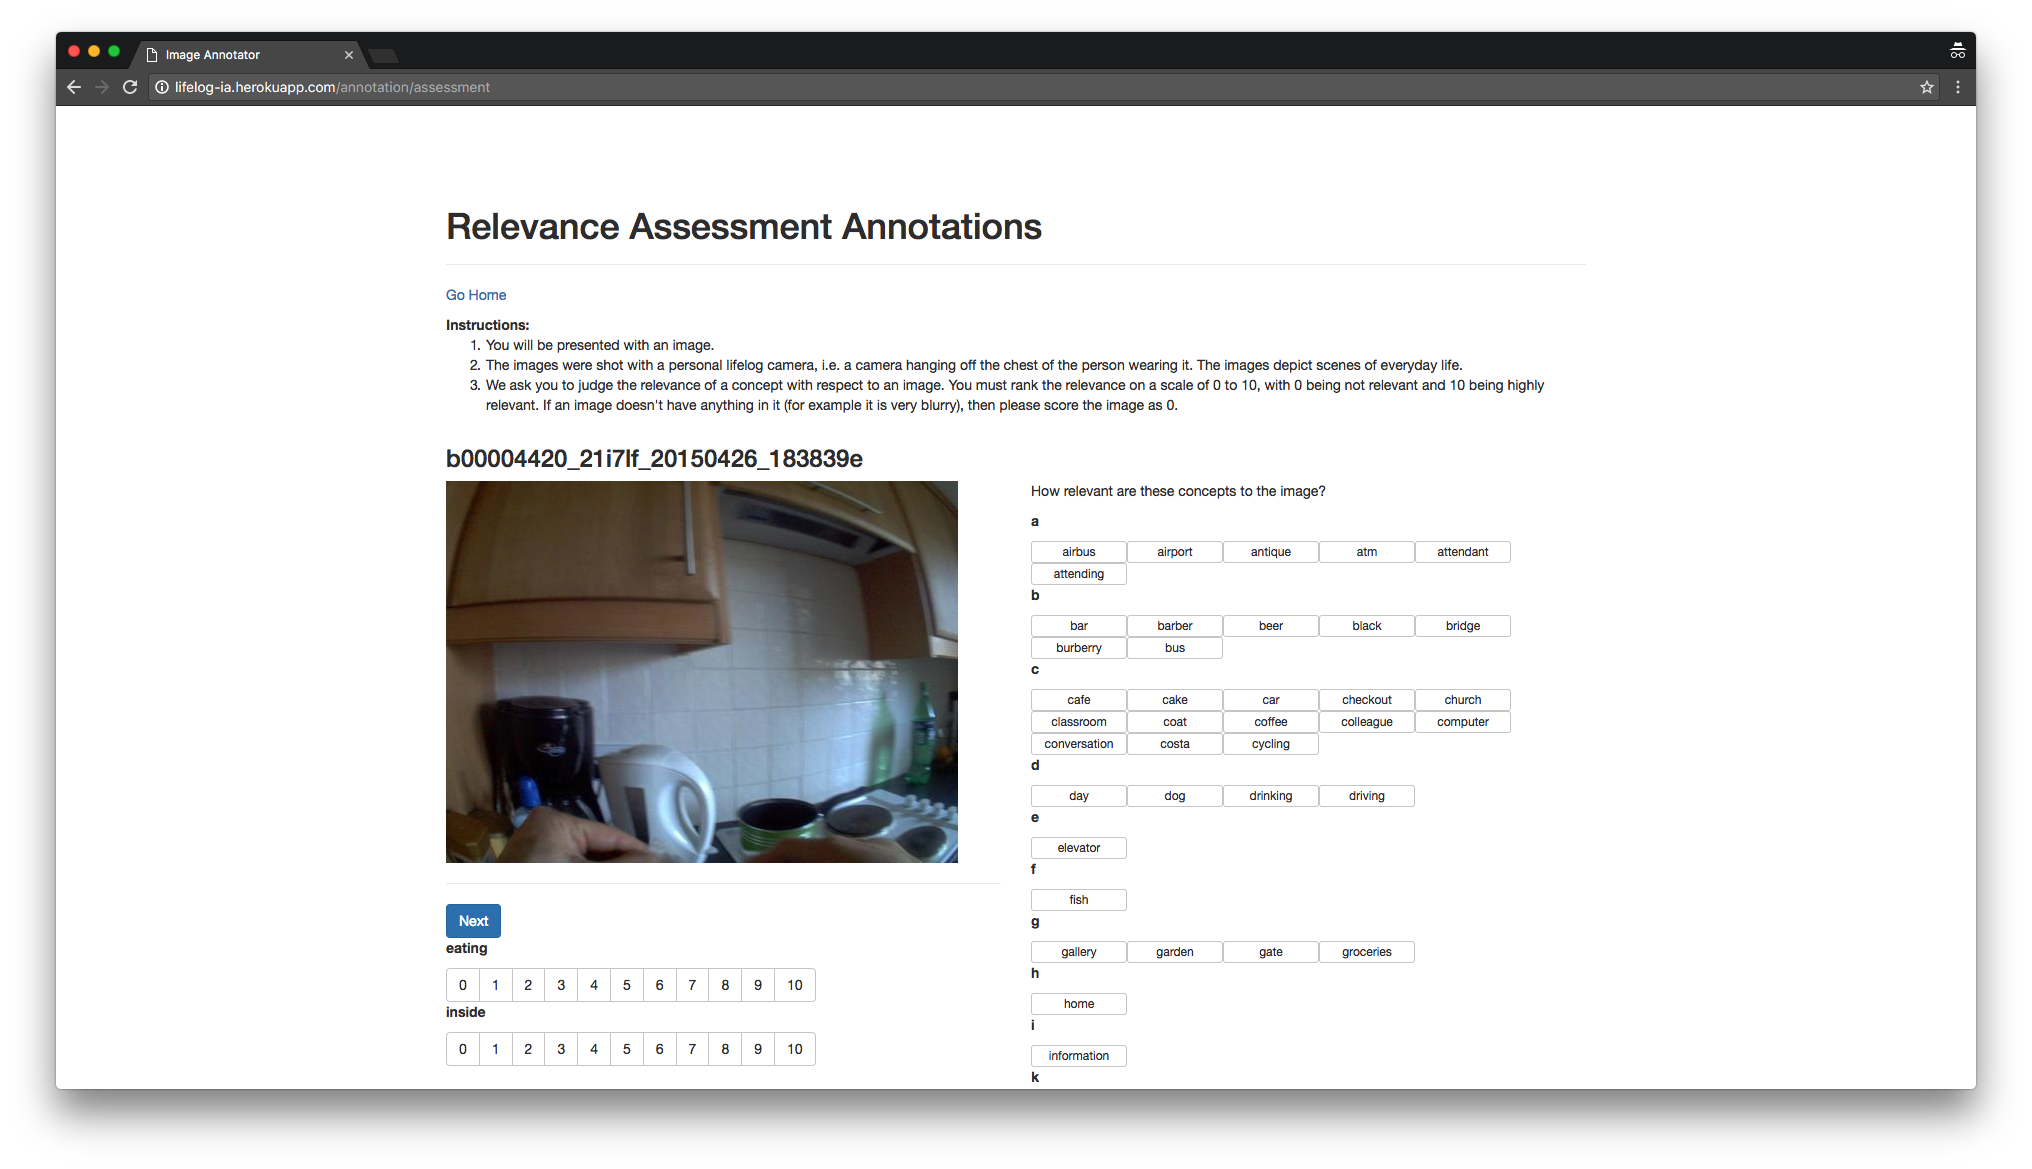
\includegraphics[width=0.95\textwidth]{images/new-rel-ass-interface}
    \caption{Updated query annotation interface}
    \label{fig:new-rel-ass}
\end{figure}

The interfaces themselves also went through many changes, both big and small. The biggest change from the initial design was for the relevance assessment interface as seen in Figure \ref{fig:new-rel-ass}. Here, each concept is grouped alphabetically; when one is clicked, assessments are added underneath the image. Here not every caption must be assessed manually. When the next button is clicked, all unassessed captions are automatically considered not relevant.

In total, there are only 6,657 images which the NTCIR-12 LSAT organisers considered to be relevant; from a collection of 88,125 images in total (only 7.5\%). If images were only annotated from the clustering method of sampling images, only 16,014 images (18\% of the data set) could be annotated. Of that, 1,176 images are considered relevant. This is why the second method of sampling images is so important -- the clusters do not provide a good distribution of relevant and non-relevant images to annotate if we just pick at random.


% - While there is an overlap of the terms in the annotations and queries, this does not necessarily mean that the terms in the annotations are used within the same context. This is particularly evident in the tag annotations. The term `key' is relevant to a query where the person wearing a lifelog camera is getting a key replaced, but the term was also found within the context of someone using a `key card' to enter their office.

% The topics were not designed to have images annotated individually out of order. Topics were designed with a range of images that are relevant, or a `moment' of images. 

% - even though images are chosen from random from a smaller pool of images, it simply was not enough to pick at random. The qrels identified 6657 images that should be relevant. From here, the pool of sampled images only contains 1179 images. Only 17.7\% of the images in the images chosen by clustering can be annotated.

The selection of image to be annotated also intuitively must impact the way a neural network captions images. If a topic contains a diverse range of locations and actions but the images sampled for annotation only cover one of these locations then it seems obvious that many images will get miscaptioned. In hindsight, taking the time to select a variety of perspectives and locations within a moment to cover edge cases might have increased the accuracy of the captions; but it is unclear by how much. It could also be the number of training examples required --- there simply may not have been enough annotations for the neural network to learn (a terrifying thought). One thing that can be said for certain is that the number of training iterations required is not the limiting factor in generating accurate captions. Over 200,000 iterations were performed for the three methodologies, and all of them got worse over time. An acceptable number of iterations for this particular setup appears to fall between 30,000 and 100,000; depending on the type of annotation.

The size of the collection and the number of manual annotations is the most likely reason the the poor performance when automatically captioning images. Take for example, the MSCOCO data set~\cite{lin2014microsoft} which contains upwards of 300,000 images with five annotations per image. The number of relevant images in each topics may also be a problem: many topics have a less than 200 relevant images associated with them (around 2\% of the actual collection). The number of images in each topic is reported in Figure \ref{fig:relevant-images}

\begin{figure}[h]
    \centering
    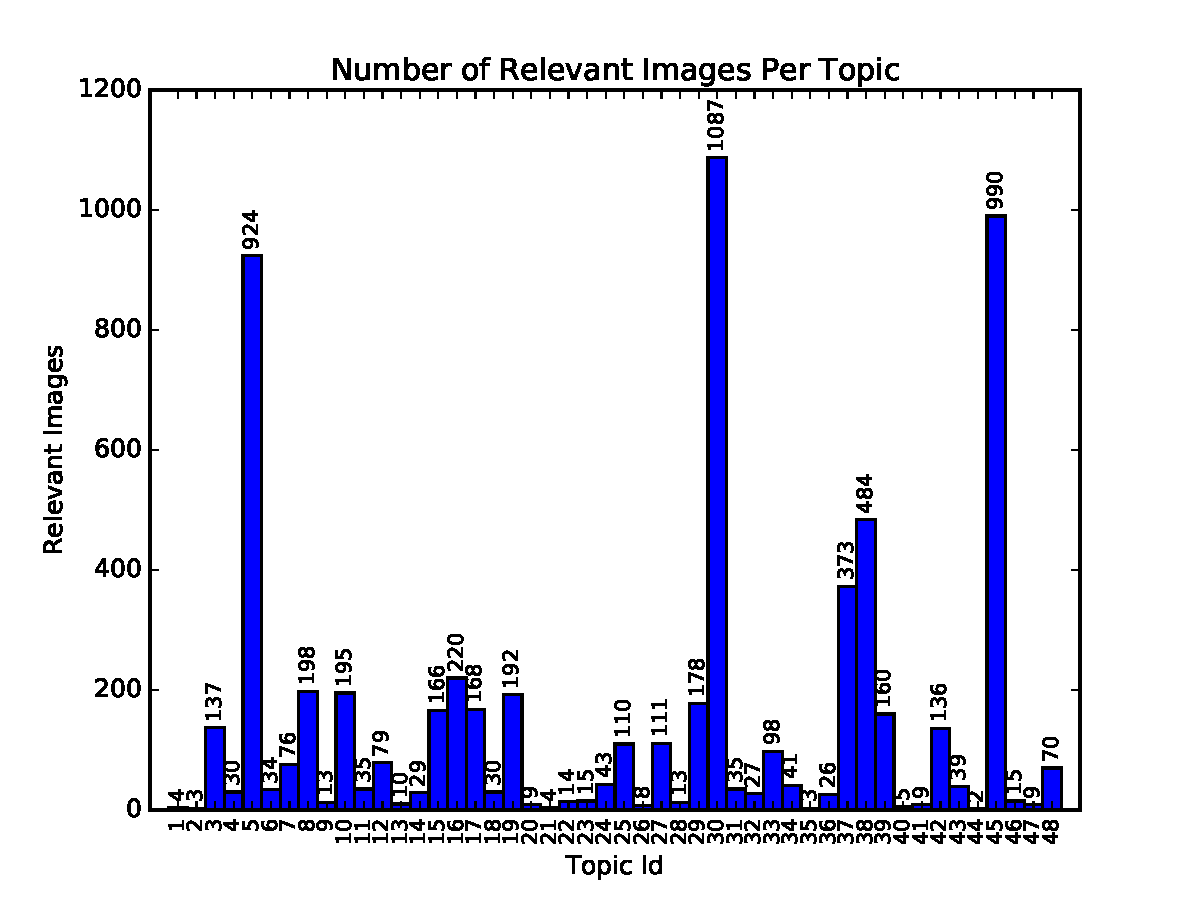
\includegraphics[width=0.95\textwidth]{graphs/relevant-images}
    \caption{Relevant images in each topic}
    \label{fig:relevant-images}
\end{figure}


% differences between each annotation methodology - All of them are very different to each other, which presents some interesting problems such as how long it takes to annotate each image, how can each annotation methodology be evaluated etc


% text
% Textual annotation are the most time consuming annotation type to collect. Many images contain two or more highly relevant events or `important' objects. Describing these can take annotators up to several minutes each. This is opposed to all the other annotation methodologies where most images can be annotated in a minute or less.

% tags
% In terms of evaluation, tags may be the opposite of textual annotations; intuitively tags should be the best at training an image classifier and are expected to perform the worst when embedded a search task. Tags, however, may be very good at boosting the performance of other annotation types in the search task when combined. For instance, searching on the text \textit{and} tags fields may increase the scores of text annotation alone.

% query
% and therefore it is unknown how well the collected queries will perform in search or for training an image classifier. The level of detail in these annotations will be very low, since most queries should be short in length.
% Much like tags, this annotation type will be very easy to collect. Formulating a query for an image should not takz a significant amount of time. There is the problem of bias \todo{Is there really? I should investigate this further}